\documentclass[sigconf]{acmart}

\usepackage{booktabs} % For formal tables

\usepackage{amsmath}
\usepackage{float}
\usepackage{hyperref}
\usepackage{listings}
\usepackage{algorithm}
\usepackage[noend]{algpseudocode}
\usepackage{graphicx}
\usepackage{courier}
\usepackage{float}
\usepackage{color}
\usepackage[margin=10pt,font=small,labelfont=bf,
  labelsep=endash]{caption}
\usepackage{ulem}

\usepackage{syntax} % for writing BNF grammar

\usepackage{forest}
\usepackage{framed}

\usepackage{tikz}
\usetikzlibrary{matrix}
\usetikzlibrary{shapes.multipart}
\usetikzlibrary{patterns}
\usetikzlibrary{positioning,fit,calc}
\usetikzlibrary{decorations.pathmorphing}
\usetikzlibrary{decorations.pathreplacing}
\usetikzlibrary{quotes}
\usetikzlibrary{graphs}
\usetikzlibrary{arrows.meta}
\usetikzlibrary{shapes}
% \usetikzlibrary{graphs,graphdrawing}
% \usegdlibrary{layered}
% \usetikzlibrary{graphdrawing,graphs,calc}
% \usegdlibrary{layered}

\usepackage{smartdiagram}

% \usetikzlibrary{external}
% \tikzexternalize % activate!
% \tikzset{external/force remake}

%% To generate figure, uncomment above three lines, and execute:
%% pdflatex -shell-escape helium.tex

\usepackage{csvsimple}
\usepackage{multirow}


\lstset{basicstyle=\footnotesize\ttfamily,breaklines=true}
% \lstset{frame=b}
\lstset{float,floatplacement=H,captionpos=b}
% \lstset{numbers=left}
\lstset{language=C}
\lstset{showstringspaces=false}
\lstset{breakindent=10pt}
% \lstset{framextopmargin=10pt}
% \lstset{framextopmargin=50pt,frame=t}
% \lstset{float=htb,language=C,frame=single, basicstyle=\small, stringstyle=\ttfamily}
% \lstset{escapeinside={(*@}{@*)}}
% \usepackage{xcolor}
\lstdefinestyle{base}{
  language=C,
  emptylines=1,
  breaklines=true,
  aboveskip=0em,
  belowskip=0em,
  % float,
  % floatplacement=H,
  basicstyle=\footnotesize\ttfamily\color{black},
  moredelim=**[is][\color{blue}]{@}{@},
  moredelim=**[is][\color{purple}]{~1}{~1},
  moredelim=**[is][\color{brown}]{~2}{~2},
  moredelim=**[is][\color{gray}]{~3}{~3},
  moredelim=**[is][\color{orange}]{~4}{~4},
  moredelim=**[is][\color{violet}]{~5}{~5},
}
\lstdefinestyle{graycode} {
  language=C,
  emptylines=1,
  breaklines=true,
  basicstyle=\footnotesize\ttfamily\color{gray!50},
  moredelim=**[is][\color{blue}]{@}{@},
}
\lstset{style=base}

\begin{document}

% \lstset{escapeinside={(*@}{@*)}}
% \lstset{style=base}




\begin{figure}[t]
  \centering
  \begin{tikzpicture}
    %% sibling distance defaults to 15mm
    \matrix[
    anchor=north west,
    column sep=2em,
    % inner sep=0em,
    % outer sep=0em
    ] {
    \node [draw] {
        \noindent\begin{minipage}{.45\linewidth}
\begin{lstlisting}[style=base, numbers=left, firstnumber=5, frame=single, framerule=0pt]
  } else if (bits & 1<<1) {
    out = bits;
    while (out & 1<<3) {
      out >>= 1;
\end{lstlisting}
          \end{minipage}
    };&
    \node [draw] {
        \noindent\begin{minipage}{.45\linewidth}
\begin{lstlisting}[style=base, numbers=left, firstnumber=5, frame=single, framerule=0pt]
  } else if (bits & 1<<1) {
    out = bits;
    while (out & 1<<2
     || out & 1<<3) {
      out >>= 1;
\end{lstlisting}
          \end{minipage}
    };\\
      \node [""] {
        \noindent\begin{minipage}{.45\linewidth}
\begin{lstlisting}[label=lst-iclones-5, style=base, numbers=left]
int main() {
  int bits, out;
  input(bits);
\end{lstlisting}
\begin{lstlisting}[label=lst-iclones-5, style=base, numbers=left, frame=single, framerule=0pt, backgroundcolor=\color{gray!10}, firstnumber=4]
  if (bits & 1) {
\end{lstlisting}
          $\qquad\cdots$
\begin{lstlisting}[style=base, numbers=left, firstnumber=5, frame=single, framerule=0pt, backgroundcolor=\color{gray!30}]
  } else if (bits & 1<<1) {
    out = bits;
    while (out & 1<<3) {
      out >>= 1;
\end{lstlisting}
          \begin{lstlisting}[style=base, numbers=left, firstnumber=9, frame=single, framerule=0pt, backgroundcolor=\color{gray!10}]
    }
  }
\end{lstlisting}
          \begin{lstlisting}[style=base, numbers=left, firstnumber=11]
  output(bits);
  output(out);
}
\end{lstlisting}
\end{minipage}
};&
\node [""] {
  \noindent\begin{minipage}{.45\linewidth}
\begin{lstlisting}[label=lst-iclones-6,style=base, numbers=left]
int main() {
  int bits, out;
  input(bits);
\end{lstlisting}
    \begin{lstlisting}[style=base, numbers=left, firstnumber=4, frame=single, framerule=0pt, backgroundcolor=\color{gray!10}]
  if (bits & 1) {
\end{lstlisting}
          $\qquad\cdots$
\begin{lstlisting}[style=base, numbers=left, firstnumber=5, frame=single, framerule=0pt, backgroundcolor=\color{gray!30}]
  } else if (bits & 1<<1) {
    out = bits;
    while (out & 1<<2
     || out & 1<<3) {
      out >>= 1;
\end{lstlisting}
    \begin{lstlisting}[style=base, numbers=left, firstnumber=10, frame=single, framerule=0pt, backgroundcolor=\color{gray!10}]
    }
  }
\end{lstlisting}
    \begin{lstlisting}[style=base, numbers=left, firstnumber=12]
  output(bits);
  output(out);
}
\end{lstlisting}
    \end{minipage}
  };\\
  \node [] {
    \begin{minipage}{.45\linewidth}
    input:\hspace{1.6mm} $bits=2$\\
    output: $out_1=2, out_2=2$\\
    \end{minipage}
  }; &
  \node [] {
    \begin{minipage}{.45\linewidth}
      input:\hspace{1.6mm} $bits = 6$\\
      output: $out_1=6, out_2=3$\\
    \end{minipage}
  }; \\
};
  \end{tikzpicture}
  \caption{Adapted from code clone reported by iClones for mdp project (https://github.com/visit1985/mdp).\label{fig:iclones-example}}
\end{figure}


\begin{figure}[t]
  \centering
  \noindent

  \begin{tikzpicture}
    % \draw [help lines, gray!30] (0,0) grid (10,10);

    \matrix (code) [anchor=west,
      draw,
      every node/.style={
        text width=6cm,
        % draw,
        inner sep=0,
        outer sep=0
      },
      "Source Code and Revision" below
      ] {
      \node {
\begin{lstlisting}[style=base, numbers=left]
int l = 0; wchar_t *c = text;
cstack_t *stack = cstack_init();
\end{lstlisting}
      };\\
      \node {
\begin{lstlisting}[style=base, frame=single, framerule=0pt, backgroundcolor=\color{gray!10}, numbers=left, firstnumber=3]
1+ if((stack->top)(stack, *c)) {
1+   if(*c == L'\\') l++;
\end{lstlisting}
      };\\
      \node {
\begin{lstlisting}[style=base, frame=single, framerule=0pt, numbers=left, firstnumber=5]
2+    (stack->pop)(stack);
\end{lstlisting}
      };\\
      \node {
\begin{lstlisting}[style=base, frame=single, framerule=0pt, backgroundcolor=\color{gray!10}, numbers=left, firstnumber=6]
1+ }
\end{lstlisting}
      };\\
      \node {
\begin{lstlisting}[style=base, frame=single, framerule=0pt, backgroundcolor=\color{gray!30}, numbers=left, firstnumber=7]
3+ else
\end{lstlisting}
      };\\
      \node {
\begin{lstlisting}[style=base, frame=single, framerule=0pt, numbers=left, firstnumber=8]
4+ if(~1strcpy(buf, stack->buf)~1) // cause
\end{lstlisting}
      };\\
      \node {
\begin{lstlisting}[style=base, frame=single, framerule=0pt, backgroundcolor=\color{gray!30}, numbers=left, firstnumber=9]
3+ {
3+  (stack->pop)(stack);
3+ }
\end{lstlisting}
      };\\
      \node {
\begin{lstlisting}[style=base, frame=single, framerule=0pt, numbers=left, firstnumber=12]
5+ else {
5+  (stack->push)(stack, *c);
5+ }
\end{lstlisting}
      };\\
    };

    % \draw (code.north) -- (10,0);

    \node (helium) [right=of code.north east, anchor=north west, "Helium Output" below] {
      \small
      \begin{tabular}{c | c | l}
        \toprule
        Commit & Dep & Closure\\
        \midrule
        1 & & \\
        2 & & 2\\
        3 & 1 & 1 3\\
        4 & 3 & 1 3 4\\
        5 & 4 & 1 3 4 5\\
        \bottomrule
      \end{tabular}
    };

    \node [right=of code.south east,
      shift={($(helium.north) - (code.north east)$)},
      anchor=south east, "Delta Debugging Conf Table" below] {
      \small
      \begin{tabular}{c|c}
        \toprule
        conf & OK?\\
        \midrule
        1 2 3 . . & $\checkmark$ \\
        . . . 4 5& $\times$ \\
        1 2 . 4 5& $\times$ \\
        . . 3 4 5& $\times$ \\
        1 2 3 4 .& $\checkmark$\\
        1 2 3 . 5& $\times$\\
        % 1 2 3 4 5& $\checkmark$\\
        
        \bottomrule
      \end{tabular}
    };
  \end{tikzpicture}
  % \begin{minipage}{.70\linewidth}
    % \end{minipage}
  \caption{Delta Debugging Example adapted from mdp project (https://github.com/visit1985/mdp).\label{fig:example-delta} }
\end{figure}





% \begin{lstlisting}
% static boolean 
% parse_time (char *argv[], int *arg_ptr)
% {
%   enum comparison_type comp;
%   const char *timearg;

%   if (COMP_LT == tval.kind) {
%     origin = options.cur_day_start;
%     if (collect_arg(argv, arg_ptr, &timearg)) {
%       get_comp_type(&timearg, &comp)
%     } else {
%     }
%   }
%   get_relative_timestamp(timearg, &tval,
%     origin, DAYSECS, errmsg);
% \end{lstlisting}

\begin{figure*}
  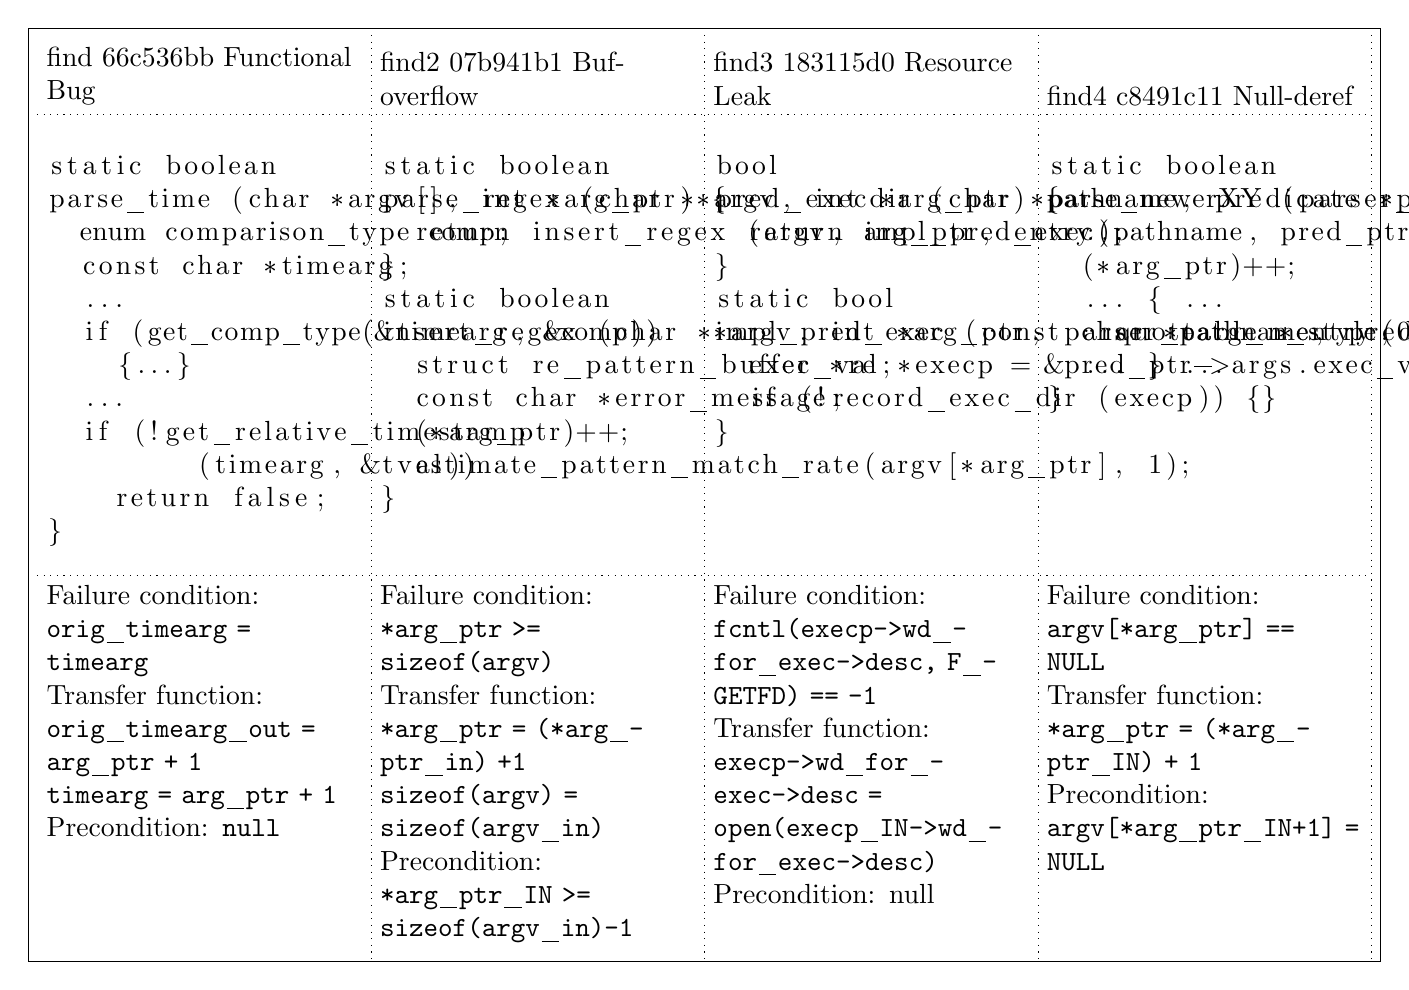
\begin{tikzpicture}
    \matrix (m) [
      draw,
      matrix anchor=north,
      every node/.style={
        % draw,
        anchor=north west, text width=4cm}] {
      \node (c1) ["find 66c536bb Functional Bug"]{
        \begin{lstlisting}
static boolean 
parse_time (char *argv[], int *arg_ptr) {
  enum comparison_type comp;
  const char *timearg;
  ...
  if (get_comp_type(&timearg, &comp))
    {...}
  ...
  if (!get_relative_timestamp
         (timearg, &tval))
    return false;
}
\end{lstlisting}
      };&
      \node (c2) ["find2 07b941b1 Buf-overflow"] {
        \begin{lstlisting}
static boolean
parse_regex (char **argv, int *arg_ptr) {
  return insert_regex (argv, arg_ptr, entry);
}
static boolean
insert_regex (char **argv, int *arg_ptr, parser_table *entry, int regex_options) {
  struct re_pattern_buffer *re;
  const char *error_message;
  (*arg_ptr)++;
  estimate_pattern_match_rate(argv[*arg_ptr], 1);
}
\end{lstlisting}
      };&
      \node (c3) ["find3 183115d0 Resource Leak"] {
        \begin{lstlisting}
bool
pred_execdir (char *pathname, predicate *pred_ptr) {
  return impl_pred_exec(pathname, pred_ptr);
}
static bool
impl_pred_exec (const char *pathname, predicate *pred_ptr) {
  exec_val *execp = &pred_ptr->args.exec_vec;
  if (!record_exec_dir (execp)) {}
}
\end{lstlisting}
      };&
      \node (c4) ["find4 c8491c11 Null-deref"] {
        \begin{lstlisting}
static boolean
parse_newerXY (parser_table* entry, char **argv, int *arg_ptr) {
  ...
  (*arg_ptr)++;
  ... { ...
    quotearg_n_style(0, options.err_quoting_style, argv[*arg_ptr]);
  ... } ...
}
\end{lstlisting}
      };\\
      \node (f1) {
        Failure condition:\\
        \texttt{orig_timearg = timearg}\\
        Transfer function:\\
        \texttt{orig_timearg_out = arg_ptr + 1}\\
        \texttt{timearg = arg_ptr + 1}\\
        Precondition: \texttt{null}\\
      };&
      \node (f2) {
        Failure condition:\\
        \texttt{*arg_ptr >= sizeof(argv)}\\
        Transfer function:\\
        \texttt{*arg_ptr = (*arg_ptr_in) +1}\\
        \texttt{sizeof(argv) = sizeof(argv_in)}\\
        Precondition: \texttt{*arg_ptr_IN >= sizeof(argv_in)-1}
      };&
      \node (f3) {
        Failure condition:\\
        \texttt{fcntl(execp->wd_for_exec->desc, F_GETFD) == -1}\\
        Transfer function:\\
        \texttt{execp->wd_for_exec->desc = open(execp_IN->wd_for_exec->desc)}\\
        Precondition: null\\
      };&
      \node (f4) {
        Failure condition:
        \texttt{argv[*arg_ptr] == NULL}\\
        Transfer function:
        \texttt{*arg_ptr = (*arg_ptr_IN) + 1}\\
        Precondition:
        \texttt{argv[*arg_ptr_IN+1] = NULL}\\
      };\\
    };
    \draw [dotted] (c1.north west) -- (c4.north east);
    \draw [dotted] (f1.north west) -- (f4.north east);
    \foreach \x in {1,2,3,4}
    \draw [dotted] (c\x.north east |- m.north) -- (f\x.south east |- m.south);
  \end{tikzpicture}
  \caption{Bug signature of four types}
\end{figure*}

% TODO \section{geneal goal of the framework}
% TODO \section{Bug Signature real example}
% TODO \section{How to compute bug signature}

\end{document}
